\section{Introduction}

On appelle modèles mixtes des modèles comportant à la fois des facteurs à effets fixes (ces effets entrant dans la définition de la moyenne du modèle) et des facteurs à effets aléatoires (ces effets entrant, quant à eux, dans la définition de la variance du modèle).

Nous allons voir dans ce projet une définition plus détaillé sur les modèles linéaire mixte (appelé aussi LMM), ainsi qu'une application en utilisant le logiciel Python. 

\section{Modèles linéaires mixtes}

La statistique traditionnelle est basé sur plusieurs hypothèses sur le maximum de vraisemblance et sur la distribution d'une loi normal. Dans un exemple de régression multiple, ces hypothèses peuvent ne pas être respecté dans le cas de non-indépendance de nos données.

Sachant que nos données son des matrices de dimension $(n\times p)$ ou $p$ représente le nombre de variables et $n$ le nombre d'observations, il peux y avoir deux types de données dans nos données:

\begin{itemize}
    \item[$\bullet$] Corrélation des variables
    \item[$\bullet$] Corrélation des observations
\end{itemize}

Dans les deux cas, l'inverse de la matrice de nécessaire à la solution du modèle linéaire est singulière, car son déterminant est proche de zéro en raison de variables ou d'observations corrélées.

Ce problème ce manifeste particulièrement quand on travail sur des données a grande dimension $(p>>n)$ quand les variables peuvent devenir redondantes et corrélées:

%$$
%\begin{array}{c}
%Y=\alpha+\beta X \\
%\beta=\left(X^{T} X\right)^{-1} X^{T} Y \\
%\left(X^{T} X\right)^{-1} \sim \frac{1}{\operatorname{det}\left(\mathrm{X}^{\mathrm{T}} \mathrm{X}\right)} \cdots \rightarrow %\infty, \quad \mathrm{n}<<\mathrm{p}
%\end{array}
%$$

Pour fixer ce problème,  on peut par exemple sélectionner des variables informatives à l'aide de l'algorithme de LASSO, ou de Ridge et en prenant en compte de la corrélations des observation à l'aide de la modélisation aléatoire dans le modèle linéaire mixte.

\subsection{Définition}
Les modèles mixtes sont une extension du modèle linéaire général qui prend en compte la structure hiérarchique des données. Ils conviennent à de nombreux types de données telles que les données groupées, les données à mesures répétées, les données longitudinales, ainsi que les combinaisons de ces trois.

On rappelle la formule du modèle de régression général:

$$
y={X \beta}+{\epsilon}
$$

ou:

\begin{itemize}
    \item[$\bullet$] $X$ est notre matrice $(N\times p)$ 
    \item[$\bullet$] $\beta$ est un vecteur colonne $p\times 1$ qui contient les coefficients de régression pour chaque variable indépendante du modèle
    \item[$\bullet$] $epsilon$ est un vecteur qui contient les erreurs (résidus) du modèle
\end{itemize}

Le modèle à effets mixtes est une extension et modélise les effets aléatoires d'une variable de regroupement:

$$
y={X \beta}+{Z u}+{\epsilon}
$$

Ou:

\begin{itemize}
    \item[$\bullet$] $Z$ est une matrice $(N\times p)$ qui contient les valeurs observées pour chaque individu $N$ pour chaque covariable $q$ des effets aléatoires.
    \item[$\bullet$] $\beta$ est un vecteur colonne $(p\times 1$)
    \item[$\bullet$] $u$ est un vecteur $(q\times 1)$ qui contient les effets aléatoires des $q$ covariables de $Z$
\end{itemize}

%Les modèles linéaires mixtes et la modélisation des effets aléatoire sont très utilisées dans divers types d'analyse de données

\newpage

\section{Application}
Les modèles linéraires mixtes doivent être utilisé lorsqu'il y a une sorte de regroupement entre les observations. 

Ici nous allons utilisé les données \textbf{"sleepstudy"} qui sont des données que l'on peut trouver dans le package \textbf{"lme4"} que l'on va exporter afin de faire notre étude avec python.

Ce jeu de données représente une étude sur le temps de réaction sur la privation de sommeil:

\begin{itemize}
    \item[$\bullet$] Au jour 0, les sujets ont dormi normalement
    
    \item[$\bullet$] À partir de cette nuit-là, ils étaient limités à 3 heures de sommeil par nuit
    
    \item[$\bullet$] Les observations représentent le temps de réaction moyen sur une série de tests donnés chaque jour à chaque sujet
\end{itemize}

Ces données proviennent de l'étude décrite dans \textit{Belenky et al.(2003)}  pour le groupe privé de sommeil et pendant les 10 premiers jours de l'étude, jusqu'à la période de récupération.

\begin{lstlisting}[language=Python]
data = pd.read_csv("C:\\Users\Walid\Documents\sleepstudy.csv")
data.index = data[data.columns[0]]
data = data[data.columns[1:4]]
\end{lstlisting}

\begin{center}
\begin{tabular}{ c c c c }
\hline
 & Reaction & Days & Subject \\
\hline
1 & 249.5600 & 0 & 308 \\
2 & 258.7047 & 1 & 308 \\
3 & 250.8006 & 2 & 308 \\
4 & 321.4398 & 3 & 308 \\
5 & 356.8519 & 4 & 308 \\
\hline
\end{tabular}
\end{center}

Notre jeu de données est constitué de 180 individus ainsi que de 3 variables:

\begin{itemize}

    \item[$\bullet$] \textbf{Reaction:} Temps de réaction en moyenne (en milisecondes)
    
    \item[$\bullet$] \textbf{Days:} Nombre de jours de privation de sommeil
    
    \item[$\bullet$] \textbf{Subject:} Numéro du sujet sur lequel l'observation a été faite.
    
\end{itemize}

\begin{figure}[H]
    \centering
    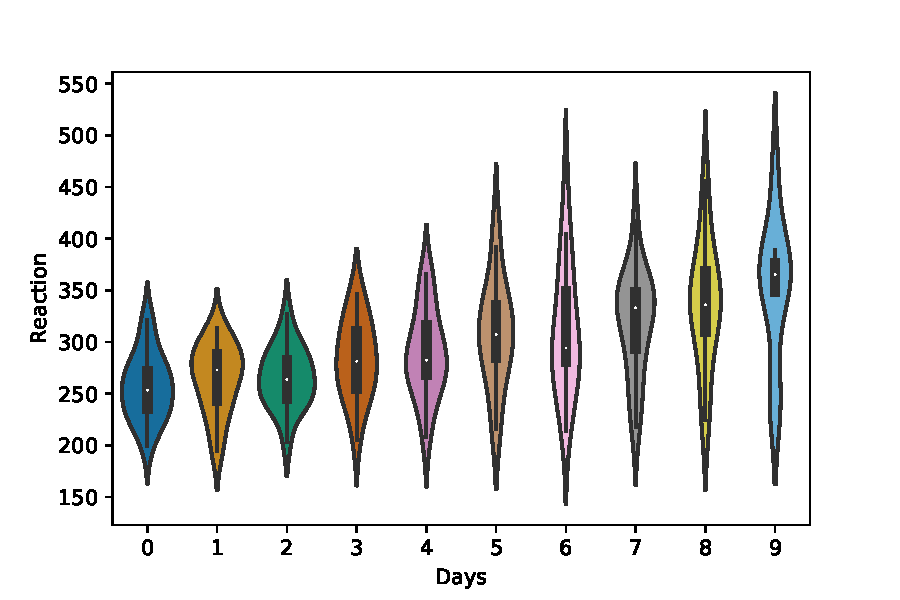
\includegraphics[width=15cm, height=7.5cm]{prebuiltimages/figure.pdf}
    \caption{violins-plots de nos données, jours /réactions.}
    %\label{fig:my_label1}
\end{figure}

On peut voir ici que plus en avance dans le temps, plus nous avons des variations en matière de temps de réactions.

\newpage

Regardons maintenant nos variables jours et temps de réactions:

\begin{figure}[H]
\centering
\begin{subfigure}{.5\textwidth}
  \centering
  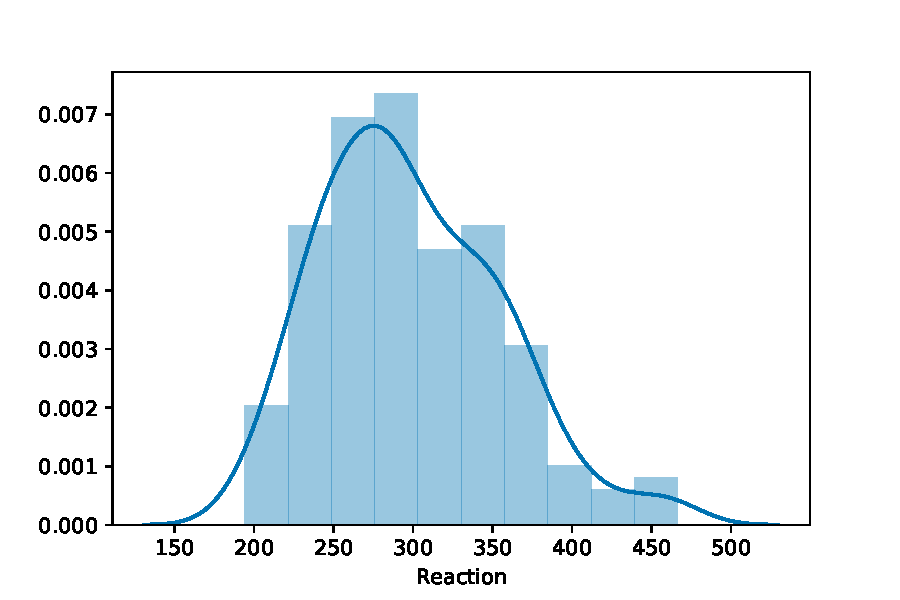
\includegraphics[width=1\linewidth]{prebuiltimages/figure3.pdf}
  \caption{Distribution des réactions}
  %\label{fig:mylabel2}
\end{subfigure}%
\begin{subfigure}{.5\textwidth}
  \centering
  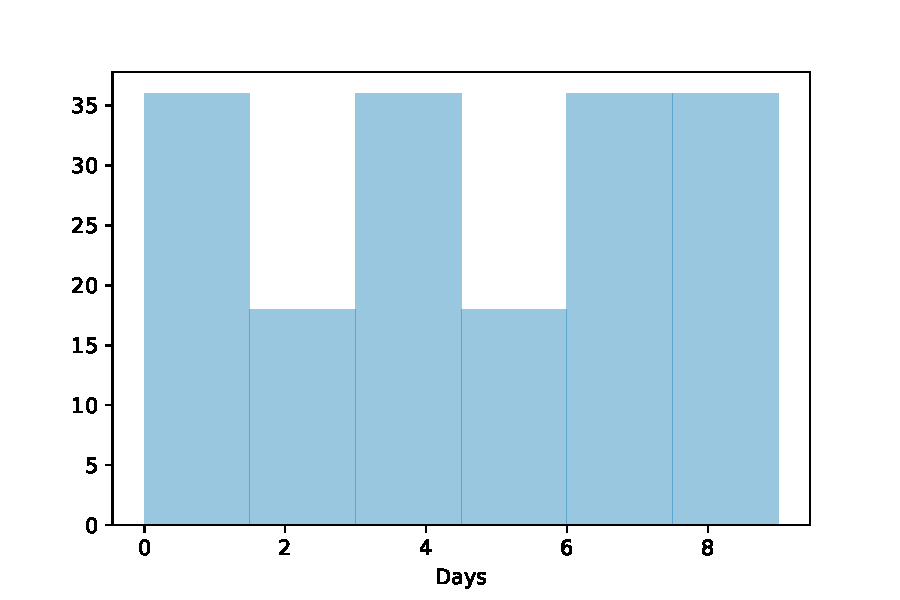
\includegraphics[width=1\linewidth]{prebuiltimages/figure4.pdf}
  \caption{Distribution des jours}
  %\label{fig:mylabel3}
\end{subfigure}
\caption{Analyse de nos variables "Reaction" et "Days"}
\label{fig:test}
\end{figure}

On remarque un temps de réactions élevé dans l'intervalle $[250,350]$ ainsi qu'un taux de privation de sommeil élevé dans les 4 derniers jours l'étude.


On regarde maintenant si le temps de réactions dépends des jours qui passent:

\begin{figure}[H]
    \centering
    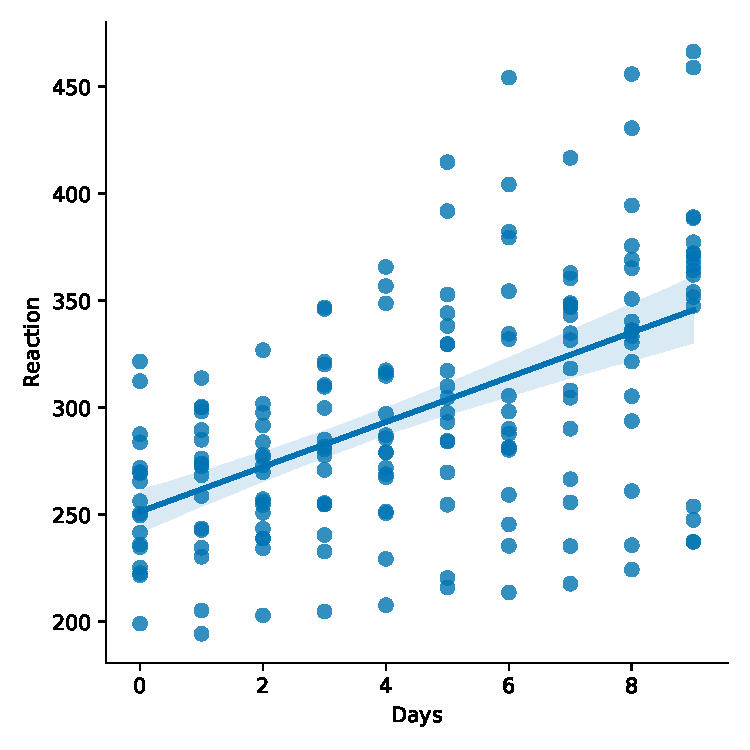
\includegraphics[width=10cm, height=7.5cm]{prebuiltimages/figure5.pdf}
    \caption{Représentation du temps de réaction en fonctions des jours}
    %\label{fig:my_label4}
\end{figure}

On remarque que le temps réaction par rapport aux jours a une tendance à la hausse avec des variations entre les jours et les individus (il existe une relation croissante  entre le temps de réaction et les jours)

\newpage

\subsection{Ordinary Least Squares (OLS) et Generalised Linear mixed Models (GLM)}

On ajuster les modéles OLS et GLM pour l'effet des jours pour chaque individu.

Le modéles OLS s'écrit:

$$
\mathrm{Y}=\beta_{0}+\Sigma_{\mathrm{j}=1 . . p} \beta_{\mathrm{j}} X_{\mathrm{j}}+\varepsilon
$$

ou:

\begin{itemize}
    \item[$\bullet$] $Y$ désigne la variable dépendante
    \item[$\bullet$] $\beta_0$ constante du modèle
    \item[$\bullet$] $X_j$ désigne la $\text{j}^{\text{ème}}$ variable explicative du modèle $(j= 1 \text{ a } p)$,
\end{itemize}

\begin{lstlisting}[language=Python]
# OLS
modelOLS = smf.ols("Reaction ~ Days", data, groups=data["Subject"])
resultOLS = modelOLS.fit()
print(resultOLS.summary())
\end{lstlisting}

Pour le modéles OLS, on obtient les résultats suivants:

\begin{center}
\begin{tabular}{ c c c c }
\multicolumn{4}{c}{OLS Regression Results} \\
\hline
\hline
Dep. Variable: & Reaction & R-squared: & 0.286\\
Model: & OLS & Adj. R-squared: & 0.282\\
Method: & Least Squares & F-statistic: & 71.46\\
Date: & Sat, 07 Nov 2020 & Prob (F-statistic): & 9.89e-15\\
Time: & 22:09:28 & Log-Likelihood: & -950.15\\
No. Observations: & 180 & AIC: & 1904.\\
Df Residuals: & 178 & BIC: & 1911.\\
Df Model: & 1 & & \\        
Covariance Type: & nonrobust & & \\
\hline
\hline
\end{tabular}
%\end{center}
%\begin{center}
\begin{tabular}{ c c c c c c }
 & Coef. & Std.Err. & z & $P>|z|$  & $[0.025  0.975]$\\
\hline
Intercept & 251.4051 & 6.610 & 38.033 & 0.000 & 238.361  264.449\\
Days & 10.4673 & 1.238 & 8.454 & 0.000 & 8.024  12.911\\
\hline
\hline
\end{tabular}
%\end{center}
%\begin{center}
\begin{tabular}{ c c c c }
Omnibus: & 1.455 & Durbin-Watson: & 0.695\\
Prob(Omnibus): & 0.483 & Jarque-Bera (JB): & 1.128\\
Skew: & 0.015 & Prob(JB): & 0.569\\
Kurtosis: & 3.387 & Cond. No. & 10.2\\
\hline
\hline
\end{tabular}
\end{center}

%\newpage

\begin{lstlisting}[language=Python]
# GLM
modelGLM = smf.glm("Reaction ~ Days", data, groups=data["Subject"])
resultGLM = modelGLM.fit()
print(resultGLM.summary())
\end{lstlisting}

Pour les modéles GLM, on obtient les résultats suivants:

\begin{center}
\begin{tabular}{ c c c c }
\multicolumn{4}{c}{Generalized Linear Model Regression Results} \\
\hline
\hline
Dep. Variable: & Reaction & No.Observations: & 180 \\
Model: & GLM & Df Residuals: & 178\\
Model Family: & Gaussian & Df Model: & 1\\
Link Function: & identity & Scale: & 2276.7\\
Method: & IRLS & Log-Likelihood: & -950.15\\
Date: & Sat, 07 Nov 2020 & Deviance: & 4.0525e+05\\
Time: & 22:13:58 & Pearson chi2: & 4.05e+05\\
No. Iterations: & 3 & & \\                                         
Covariance Type: & nonrobust & & \\
\end{tabular}
%\end{center}
%\begin{center}
\begin{tabular}{ c c c c c c }
\hline
 & Coef. & Std.Err. & z & $P>|z|$  & $[0.025  0.975]$\\
\hline
Intercept & 251.4051 & 6.610 & 38.033 & 0.000 & 238.449  264.361\\
Days & 10.4673 & 1.238 & 8.454 & 0.000 & 8.040  12.894\\
\hline
\hline
\end{tabular}
\end{center}

\newpage

\subsection{LMM}

Maintenant, pour ajuster un modèle d'interception aléatoire, rappelez-vous que ce type de modèle permet à différents clusters (un groupe) d'avoir des interceptions différentes

\begin{lstlisting}[language=Python]
#LMM
md = smf.mixedlm("Reaction ~ Days", data, groups=data["Subject"])
mdf = md.fit()
print(mdf.summary())
\end{lstlisting}

On obtient les résultats suivants:

\begin{center}
\begin{tabular}{ c c c c }
\multicolumn{4}{c}{Mixed Linear Model Regression Results} \\
\hline
\hline
Model: & MixedLM & Dependent Variable: & Reaction \\
No. Observations: & 180 & Method: & REML\\     
No. Groups: & 18 & Scale: & 960.4568\\
Min. group size: & 10 & Log-Likelihood: & -893.2325\\
Max. group size: & 10 & Converged: & Yes\\
Mean group size: & 10.0 & &
\end{tabular}
%\end{center}
%\begin{center}
\begin{tabular}{ c c c c c c }
\hline
 & Coef. & Std.Err. & z & $P>|z|$  & $[0.025  0.975]$\\
\hline
Intercept & 251.405 & 9.747 & 25.794 & 0.000 & 232.302 270.508\\
Days & 10.467 & 0.804 & 13.015 & 0.000 & 8.891  12.044\\
Group Var & 1378.176 & 17.156 & & & \\
\hline
\hline
\end{tabular}
\end{center}

On remarque que:

\begin{itemize}
    \item[$\bullet$] Le nombre de groupes = 18
    \item[$\bullet$] Corrélation des observations
\end{itemize}

En calculant l'erreur quadratique moyenne, on obtient les résultats suivants:

\begin{lstlisting}[language=Python]
y = data.Reaction
y_predict_LMM = resultLMM.fittedvalues
RMSE_LMM = sqrt(((y-y_predict_LMM)**2).values.mean())
results = pd.DataFrame()
results["Method"] = ["LMM"]
results["RMSE"] = RMSE_LMM
y_predict_GLM = resultGLM.fittedvalues
RMSE_GLM = sqrt(((y-y_predict_GLM)**2).values.mean())
results.loc[1] = ["GLM",RMSE_GLM]
y_predict_OLS = resultOLS.fittedvalues
RMSE_OLS = sqrt(((y-y_predict_OLS)**2).values.mean())
results.loc[2] = ["OLS",RMSE_OLS]
results
\end{lstlisting}

\begin{center}
\begin{tabular}{ c c }
\hline
Method & RMSE\\
\hline
LMM	& 29.410624\\
GLM	& 47.448898\\
OLS	& 47.448898\\
\hline
\end{tabular}
\end{center}

On remarque que l'erreur quadratique moyenne du LMM est la plus petite, ce qui montre que cette méthode fourni un meilleur ajustement que les deux autres méthodes.

\newpage

\begin{lstlisting}[language=Python]
performance = pd.DataFrame()
performance["residuals"] = resultLMM.resid.values
performance["Days"] = data.Days
performance["predicted"] = resultLMM.fittedvalues
sns.lmplot(x = "predicted", y = "residuals", data = performance)
plt.savefig("figure6.pdf") 
\end{lstlisting}

\begin{figure}[H]
    \centering
    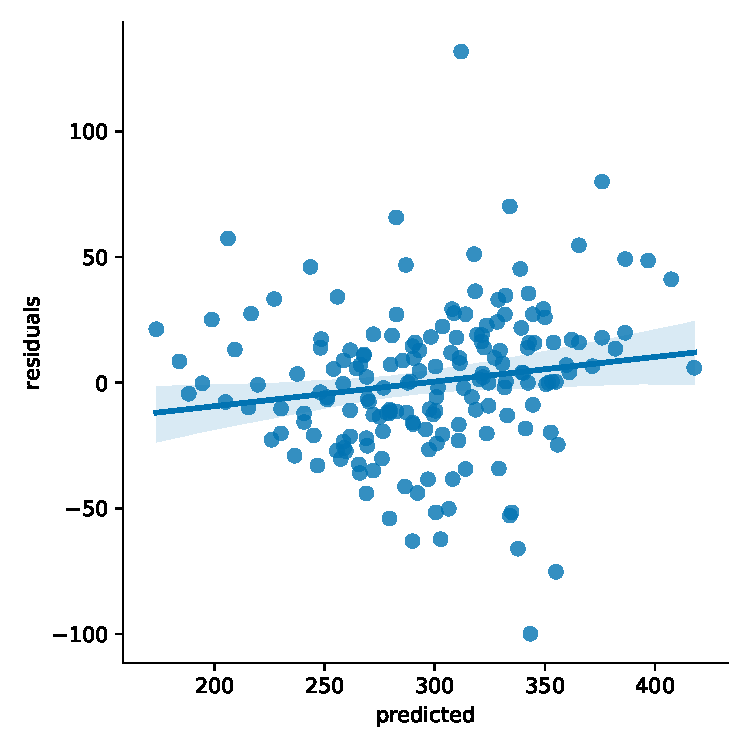
\includegraphics[width=10cm, height=7.5cm]{prebuiltimages/figure6.pdf}
    \caption{Représentation du temps de réactions en fonctions des jours après ajustement LMM}
    %\label{fig:my_label4}
\end{figure}

Grâce a cette méthode, les résidus sont bien meilleurs qu'avant (le temps de réactions étant mieux répartis en fonction des jours)

\section{Conclusion}
Nous avons appris que le modèle linéaire mixte est utilisé pour tenir compte de la non-indépendance et donc de la non-normalité des données.


le modèle fourni généralement un meilleur ajustement et expliquent plus de variation dans les données comparé aux modéles OLS ou GLM.

\begin{thebibliography}{99}
\bibitem{1} How Linear Mixed Model Works (Nikolay Oskolkov)\\
{\it https://towardsdatascience.com/how-linear-mixed-model-works-350950a82911}

\bibitem{2} How Linear Mixed Model Works (Nikolay Oskolkov)\\
{\it https://www.statsmodels.org/stable/mixed$\_$linear.html}

\bibitem{3} mixed$\_$models (OJ Watson)\\
{\it https://www.kaggle.com/ojwatson/mixed-models}
\end{thebibliography}

\newpage


